% Created by tikzDevice version 0.12.6 on 2026-07-05 17:37:31
% !TEX encoding = UTF-8 Unicode
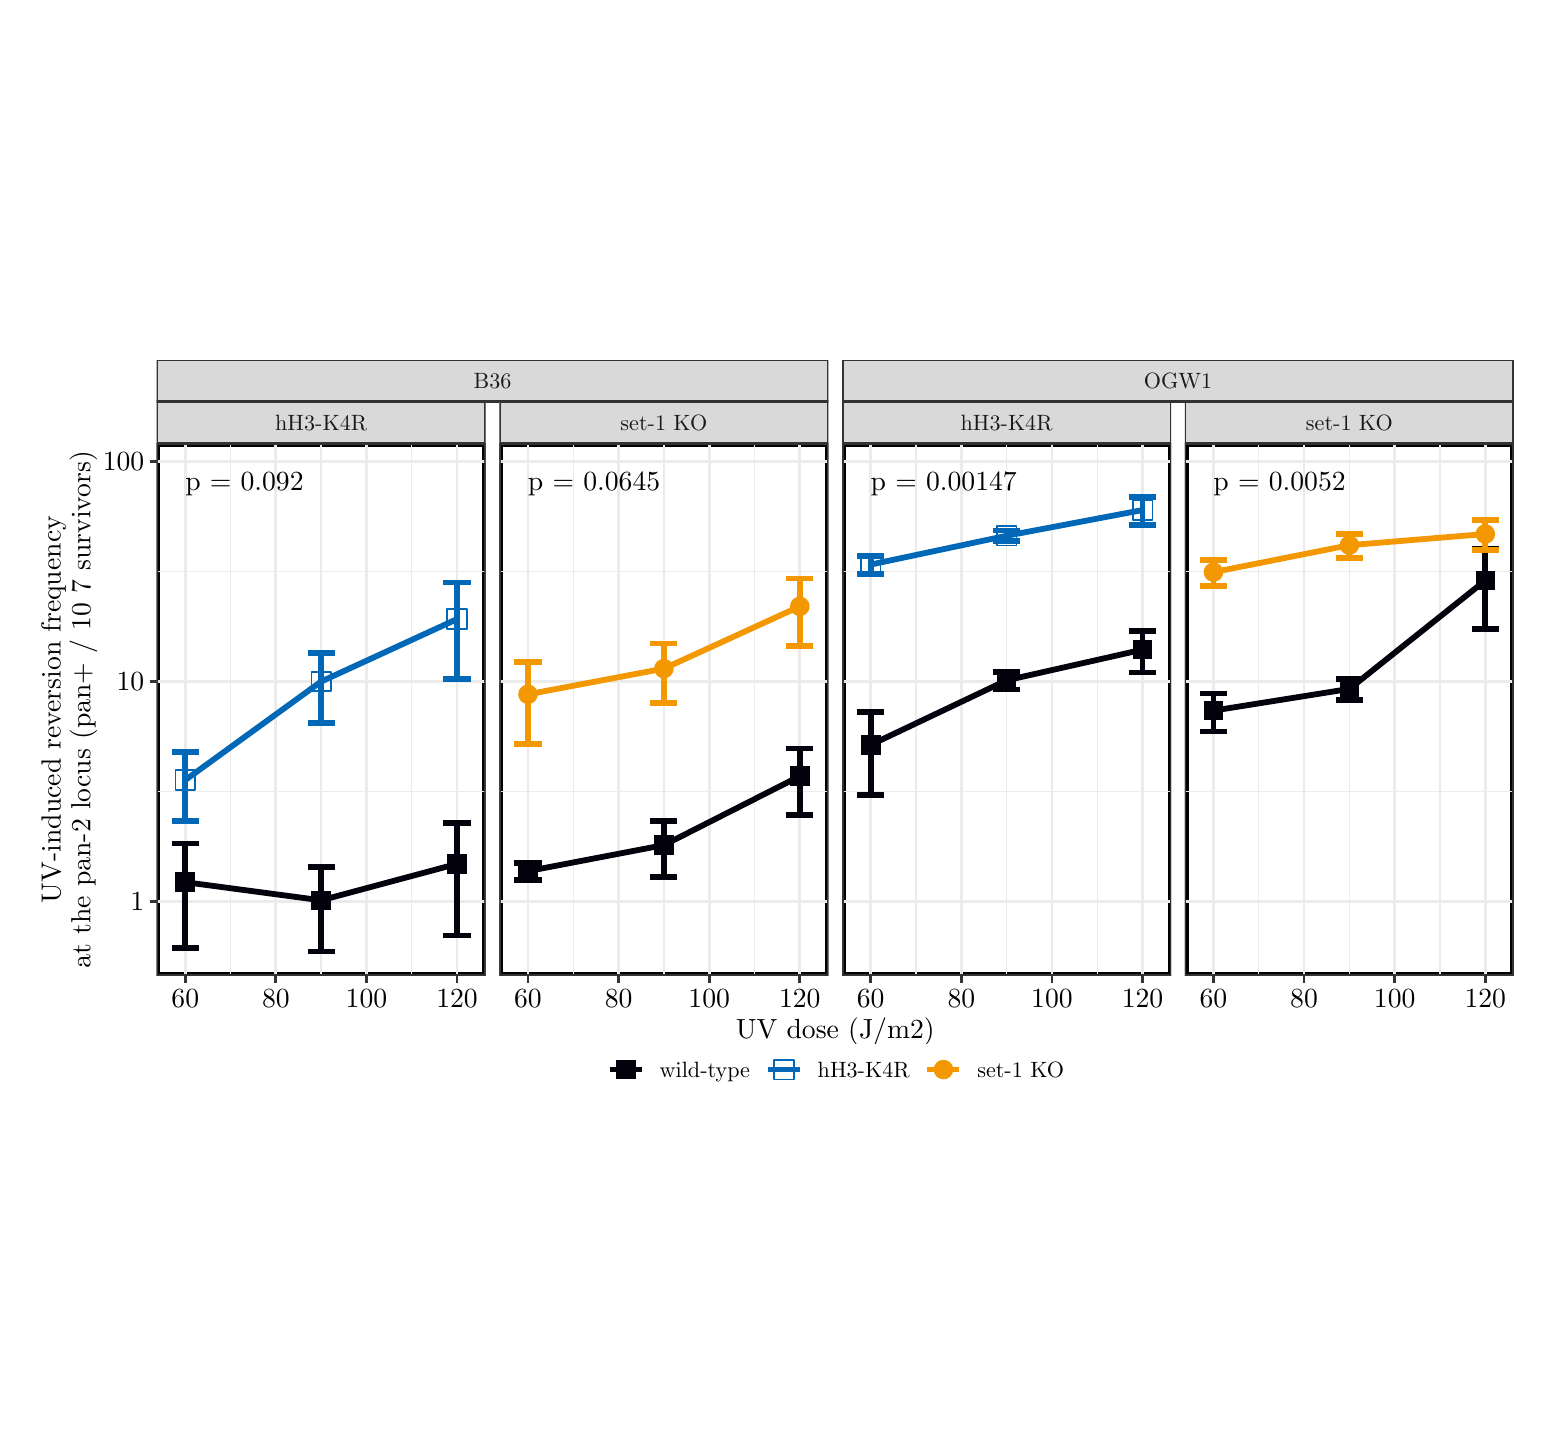
\begin{tikzpicture}[x=1pt,y=1pt]
\definecolor{fillColor}{RGB}{255,255,255}
\path[use as bounding box,fill=fillColor,fill opacity=0.00] (0,0) rectangle (542.02,505.89);
\begin{scope}
\path[clip] (  0.00,115.13) rectangle (542.02,390.76);
\definecolor{drawColor}{RGB}{255,255,255}
\definecolor{fillColor}{RGB}{255,255,255}

\path[draw=drawColor,line width= 1.0pt,line join=round,line cap=round,fill=fillColor] (  0.00,115.13) rectangle (542.03,390.76);
\end{scope}
\begin{scope}
\path[clip] ( 46.63,163.33) rectangle (165.48,355.63);
\definecolor{drawColor}{RGB}{0,0,0}
\definecolor{fillColor}{RGB}{255,255,255}

\path[draw=drawColor,line width= 2.6pt,line join=round,line cap=round,fill=fillColor] ( 46.63,163.33) rectangle (165.48,355.63);
\definecolor{drawColor}{gray}{0.92}

\path[draw=drawColor,line width= 0.5pt,line join=round] ( 46.63,229.92) --
	(165.48,229.92);

\path[draw=drawColor,line width= 0.5pt,line join=round] ( 46.63,309.44) --
	(165.48,309.44);

\path[draw=drawColor,line width= 0.5pt,line join=round] ( 73.31,163.33) --
	( 73.31,355.63);

\path[draw=drawColor,line width= 0.5pt,line join=round] (106.05,163.33) --
	(106.05,355.63);

\path[draw=drawColor,line width= 0.5pt,line join=round] (138.79,163.33) --
	(138.79,355.63);

\path[draw=drawColor,line width= 1.0pt,line join=round] ( 46.63,190.17) --
	(165.48,190.17);

\path[draw=drawColor,line width= 1.0pt,line join=round] ( 46.63,269.68) --
	(165.48,269.68);

\path[draw=drawColor,line width= 1.0pt,line join=round] ( 46.63,349.19) --
	(165.48,349.19);

\path[draw=drawColor,line width= 1.0pt,line join=round] ( 56.94,163.33) --
	( 56.94,355.63);

\path[draw=drawColor,line width= 1.0pt,line join=round] ( 89.68,163.33) --
	( 89.68,355.63);

\path[draw=drawColor,line width= 1.0pt,line join=round] (122.42,163.33) --
	(122.42,355.63);

\path[draw=drawColor,line width= 1.0pt,line join=round] (155.16,163.33) --
	(155.16,355.63);
\definecolor{drawColor}{RGB}{2,1,12}

\path[draw=drawColor,line width= 2.1pt,line join=round] ( 56.94,197.11) --
	(106.05,190.56) --
	(155.16,203.73);
\definecolor{drawColor}{RGB}{0,104,183}

\path[draw=drawColor,line width= 2.1pt,line join=round] ( 56.94,234.01) --
	(106.05,269.61) --
	(155.16,292.18);
\definecolor{fillColor}{RGB}{2,1,12}

\path[fill=fillColor] ( 53.40,193.57) --
	( 60.48,193.57) --
	( 60.48,200.65) --
	( 53.40,200.65) --
	cycle;

\path[fill=fillColor] (102.52,187.03) --
	(109.59,187.03) --
	(109.59,194.10) --
	(102.52,194.10) --
	cycle;

\path[fill=fillColor] (151.63,200.20) --
	(158.70,200.20) --
	(158.70,207.27) --
	(151.63,207.27) --
	cycle;

\path[draw=drawColor,line width= 0.6pt,line join=round,line cap=round] ( 53.40,230.47) rectangle ( 60.48,237.54);

\path[draw=drawColor,line width= 0.6pt,line join=round,line cap=round] (102.52,266.08) rectangle (109.59,273.15);

\path[draw=drawColor,line width= 0.6pt,line join=round,line cap=round] (151.63,288.65) rectangle (158.70,295.72);
\definecolor{drawColor}{RGB}{2,1,12}

\path[draw=drawColor,line width= 2.1pt,line join=round] ( 52.03,211.06) --
	( 61.85,211.06);

\path[draw=drawColor,line width= 2.1pt,line join=round] ( 56.94,211.06) --
	( 56.94,173.34);

\path[draw=drawColor,line width= 2.1pt,line join=round] ( 52.03,173.34) --
	( 61.85,173.34);

\path[draw=drawColor,line width= 2.1pt,line join=round] (101.14,202.54) --
	(110.96,202.54);

\path[draw=drawColor,line width= 2.1pt,line join=round] (106.05,202.54) --
	(106.05,172.07);

\path[draw=drawColor,line width= 2.1pt,line join=round] (101.14,172.07) --
	(110.96,172.07);

\path[draw=drawColor,line width= 2.1pt,line join=round] (150.25,218.36) --
	(160.07,218.36);

\path[draw=drawColor,line width= 2.1pt,line join=round] (155.16,218.36) --
	(155.16,177.86);

\path[draw=drawColor,line width= 2.1pt,line join=round] (150.25,177.86) --
	(160.07,177.86);
\definecolor{drawColor}{RGB}{0,104,183}

\path[draw=drawColor,line width= 2.1pt,line join=round] ( 52.03,244.29) --
	( 61.85,244.29);

\path[draw=drawColor,line width= 2.1pt,line join=round] ( 56.94,244.29) --
	( 56.94,219.29);

\path[draw=drawColor,line width= 2.1pt,line join=round] ( 52.03,219.29) --
	( 61.85,219.29);

\path[draw=drawColor,line width= 2.1pt,line join=round] (101.14,280.00) --
	(110.96,280.00);

\path[draw=drawColor,line width= 2.1pt,line join=round] (106.05,280.00) --
	(106.05,254.69);

\path[draw=drawColor,line width= 2.1pt,line join=round] (101.14,254.69) --
	(110.96,254.69);

\path[draw=drawColor,line width= 2.1pt,line join=round] (150.25,305.40) --
	(160.07,305.40);

\path[draw=drawColor,line width= 2.1pt,line join=round] (155.16,305.40) --
	(155.16,270.49);

\path[draw=drawColor,line width= 2.1pt,line join=round] (150.25,270.49) --
	(160.07,270.49);
\definecolor{drawColor}{RGB}{0,0,0}

\node[text=drawColor,anchor=base west,inner sep=0pt, outer sep=0pt, scale=  1.00] at ( 56.94,338.70) {p = 0.092};
\definecolor{drawColor}{gray}{0.20}

\path[draw=drawColor,line width= 1.0pt,line join=round,line cap=round] ( 46.63,163.33) rectangle (165.48,355.63);
\end{scope}
\begin{scope}
\path[clip] (170.48,163.33) rectangle (289.33,355.63);
\definecolor{drawColor}{RGB}{0,0,0}
\definecolor{fillColor}{RGB}{255,255,255}

\path[draw=drawColor,line width= 2.6pt,line join=round,line cap=round,fill=fillColor] (170.48,163.33) rectangle (289.33,355.63);
\definecolor{drawColor}{gray}{0.92}

\path[draw=drawColor,line width= 0.5pt,line join=round] (170.48,229.92) --
	(289.33,229.92);

\path[draw=drawColor,line width= 0.5pt,line join=round] (170.48,309.44) --
	(289.33,309.44);

\path[draw=drawColor,line width= 0.5pt,line join=round] (197.16,163.33) --
	(197.16,355.63);

\path[draw=drawColor,line width= 0.5pt,line join=round] (229.90,163.33) --
	(229.90,355.63);

\path[draw=drawColor,line width= 0.5pt,line join=round] (262.64,163.33) --
	(262.64,355.63);

\path[draw=drawColor,line width= 1.0pt,line join=round] (170.48,190.17) --
	(289.33,190.17);

\path[draw=drawColor,line width= 1.0pt,line join=round] (170.48,269.68) --
	(289.33,269.68);

\path[draw=drawColor,line width= 1.0pt,line join=round] (170.48,349.19) --
	(289.33,349.19);

\path[draw=drawColor,line width= 1.0pt,line join=round] (180.79,163.33) --
	(180.79,355.63);

\path[draw=drawColor,line width= 1.0pt,line join=round] (213.53,163.33) --
	(213.53,355.63);

\path[draw=drawColor,line width= 1.0pt,line join=round] (246.27,163.33) --
	(246.27,355.63);

\path[draw=drawColor,line width= 1.0pt,line join=round] (279.01,163.33) --
	(279.01,355.63);
\definecolor{drawColor}{RGB}{2,1,12}

\path[draw=drawColor,line width= 2.1pt,line join=round] (180.79,201.11) --
	(229.90,210.51) --
	(279.01,235.43);
\definecolor{drawColor}{RGB}{243,152,0}

\path[draw=drawColor,line width= 2.1pt,line join=round] (180.79,264.99) --
	(229.90,274.29) --
	(279.01,296.77);
\definecolor{fillColor}{RGB}{2,1,12}

\path[fill=fillColor] (177.25,197.58) --
	(184.33,197.58) --
	(184.33,204.65) --
	(177.25,204.65) --
	cycle;

\path[fill=fillColor] (226.37,206.97) --
	(233.44,206.97) --
	(233.44,214.05) --
	(226.37,214.05) --
	cycle;

\path[fill=fillColor] (275.48,231.89) --
	(282.55,231.89) --
	(282.55,238.96) --
	(275.48,238.96) --
	cycle;
\definecolor{fillColor}{RGB}{243,152,0}

\path[fill=fillColor] (180.79,264.99) circle (  3.54);

\path[fill=fillColor] (229.90,274.29) circle (  3.54);

\path[fill=fillColor] (279.01,296.77) circle (  3.54);
\definecolor{drawColor}{RGB}{2,1,12}

\path[draw=drawColor,line width= 2.1pt,line join=round] (175.88,204.06) --
	(185.70,204.06);

\path[draw=drawColor,line width= 2.1pt,line join=round] (180.79,204.06) --
	(180.79,197.89);

\path[draw=drawColor,line width= 2.1pt,line join=round] (175.88,197.89) --
	(185.70,197.89);

\path[draw=drawColor,line width= 2.1pt,line join=round] (224.99,219.10) --
	(234.81,219.10);

\path[draw=drawColor,line width= 2.1pt,line join=round] (229.90,219.10) --
	(229.90,199.04);

\path[draw=drawColor,line width= 2.1pt,line join=round] (224.99,199.04) --
	(234.81,199.04);

\path[draw=drawColor,line width= 2.1pt,line join=round] (274.10,245.44) --
	(283.92,245.44);

\path[draw=drawColor,line width= 2.1pt,line join=round] (279.01,245.44) --
	(279.01,221.26);

\path[draw=drawColor,line width= 2.1pt,line join=round] (274.10,221.26) --
	(283.92,221.26);
\definecolor{drawColor}{RGB}{243,152,0}

\path[draw=drawColor,line width= 2.1pt,line join=round] (175.88,276.78) --
	(185.70,276.78);

\path[draw=drawColor,line width= 2.1pt,line join=round] (180.79,276.78) --
	(180.79,246.93);

\path[draw=drawColor,line width= 2.1pt,line join=round] (175.88,246.93) --
	(185.70,246.93);

\path[draw=drawColor,line width= 2.1pt,line join=round] (224.99,283.39) --
	(234.81,283.39);

\path[draw=drawColor,line width= 2.1pt,line join=round] (229.90,283.39) --
	(229.90,261.90);

\path[draw=drawColor,line width= 2.1pt,line join=round] (224.99,261.90) --
	(234.81,261.90);

\path[draw=drawColor,line width= 2.1pt,line join=round] (274.10,306.87) --
	(283.92,306.87);

\path[draw=drawColor,line width= 2.1pt,line join=round] (279.01,306.87) --
	(279.01,282.46);

\path[draw=drawColor,line width= 2.1pt,line join=round] (274.10,282.46) --
	(283.92,282.46);
\definecolor{drawColor}{RGB}{0,0,0}

\node[text=drawColor,anchor=base west,inner sep=0pt, outer sep=0pt, scale=  1.00] at (180.79,338.70) {p = 0.0645};
\definecolor{drawColor}{gray}{0.20}

\path[draw=drawColor,line width= 1.0pt,line join=round,line cap=round] (170.48,163.33) rectangle (289.33,355.63);
\end{scope}
\begin{scope}
\path[clip] (294.33,163.33) rectangle (413.18,355.63);
\definecolor{drawColor}{RGB}{0,0,0}
\definecolor{fillColor}{RGB}{255,255,255}

\path[draw=drawColor,line width= 2.6pt,line join=round,line cap=round,fill=fillColor] (294.33,163.33) rectangle (413.18,355.63);
\definecolor{drawColor}{gray}{0.92}

\path[draw=drawColor,line width= 0.5pt,line join=round] (294.33,229.92) --
	(413.18,229.92);

\path[draw=drawColor,line width= 0.5pt,line join=round] (294.33,309.44) --
	(413.18,309.44);

\path[draw=drawColor,line width= 0.5pt,line join=round] (321.01,163.33) --
	(321.01,355.63);

\path[draw=drawColor,line width= 0.5pt,line join=round] (353.75,163.33) --
	(353.75,355.63);

\path[draw=drawColor,line width= 0.5pt,line join=round] (386.49,163.33) --
	(386.49,355.63);

\path[draw=drawColor,line width= 1.0pt,line join=round] (294.33,190.17) --
	(413.18,190.17);

\path[draw=drawColor,line width= 1.0pt,line join=round] (294.33,269.68) --
	(413.18,269.68);

\path[draw=drawColor,line width= 1.0pt,line join=round] (294.33,349.19) --
	(413.18,349.19);

\path[draw=drawColor,line width= 1.0pt,line join=round] (304.64,163.33) --
	(304.64,355.63);

\path[draw=drawColor,line width= 1.0pt,line join=round] (337.38,163.33) --
	(337.38,355.63);

\path[draw=drawColor,line width= 1.0pt,line join=round] (370.12,163.33) --
	(370.12,355.63);

\path[draw=drawColor,line width= 1.0pt,line join=round] (402.86,163.33) --
	(402.86,355.63);
\definecolor{drawColor}{RGB}{2,1,12}

\path[draw=drawColor,line width= 2.1pt,line join=round] (304.64,246.74) --
	(353.75,270.06) --
	(402.86,281.13);
\definecolor{drawColor}{RGB}{0,104,183}

\path[draw=drawColor,line width= 2.1pt,line join=round] (304.64,311.88) --
	(353.75,322.29) --
	(402.86,331.58);
\definecolor{fillColor}{RGB}{2,1,12}

\path[fill=fillColor] (301.10,243.21) --
	(308.18,243.21) --
	(308.18,250.28) --
	(301.10,250.28) --
	cycle;

\path[fill=fillColor] (350.21,266.52) --
	(357.29,266.52) --
	(357.29,273.60) --
	(350.21,273.60) --
	cycle;

\path[fill=fillColor] (399.33,277.59) --
	(406.40,277.59) --
	(406.40,284.66) --
	(399.33,284.66) --
	cycle;

\path[draw=drawColor,line width= 0.6pt,line join=round,line cap=round] (301.10,308.34) rectangle (308.18,315.42);

\path[draw=drawColor,line width= 0.6pt,line join=round,line cap=round] (350.21,318.76) rectangle (357.29,325.83);

\path[draw=drawColor,line width= 0.6pt,line join=round,line cap=round] (399.33,328.04) rectangle (406.40,335.11);
\definecolor{drawColor}{RGB}{2,1,12}

\path[draw=drawColor,line width= 2.1pt,line join=round] (299.73,258.53) --
	(309.55,258.53);

\path[draw=drawColor,line width= 2.1pt,line join=round] (304.64,258.53) --
	(304.64,228.72);

\path[draw=drawColor,line width= 2.1pt,line join=round] (299.73,228.72) --
	(309.55,228.72);

\path[draw=drawColor,line width= 2.1pt,line join=round] (348.84,273.10) --
	(358.66,273.10);

\path[draw=drawColor,line width= 2.1pt,line join=round] (353.75,273.10) --
	(353.75,266.72);

\path[draw=drawColor,line width= 2.1pt,line join=round] (348.84,266.72) --
	(358.66,266.72);

\path[draw=drawColor,line width= 2.1pt,line join=round] (397.95,287.79) --
	(407.77,287.79);

\path[draw=drawColor,line width= 2.1pt,line join=round] (402.86,287.79) --
	(402.86,272.87);

\path[draw=drawColor,line width= 2.1pt,line join=round] (397.95,272.87) --
	(407.77,272.87);
\definecolor{drawColor}{RGB}{0,104,183}

\path[draw=drawColor,line width= 2.1pt,line join=round] (299.73,314.98) --
	(309.55,314.98);

\path[draw=drawColor,line width= 2.1pt,line join=round] (304.64,314.98) --
	(304.64,308.48);

\path[draw=drawColor,line width= 2.1pt,line join=round] (299.73,308.48) --
	(309.55,308.48);

\path[draw=drawColor,line width= 2.1pt,line join=round] (348.84,324.19) --
	(358.66,324.19);

\path[draw=drawColor,line width= 2.1pt,line join=round] (353.75,324.19) --
	(353.75,320.29);

\path[draw=drawColor,line width= 2.1pt,line join=round] (348.84,320.29) --
	(358.66,320.29);

\path[draw=drawColor,line width= 2.1pt,line join=round] (397.95,336.15) --
	(407.77,336.15);

\path[draw=drawColor,line width= 2.1pt,line join=round] (402.86,336.15) --
	(402.86,326.31);

\path[draw=drawColor,line width= 2.1pt,line join=round] (397.95,326.31) --
	(407.77,326.31);
\definecolor{drawColor}{RGB}{0,0,0}

\node[text=drawColor,anchor=base west,inner sep=0pt, outer sep=0pt, scale=  1.00] at (304.64,338.70) {p = 0.00147};
\definecolor{drawColor}{gray}{0.20}

\path[draw=drawColor,line width= 1.0pt,line join=round,line cap=round] (294.33,163.33) rectangle (413.18,355.63);
\end{scope}
\begin{scope}
\path[clip] (418.18,163.33) rectangle (537.02,355.63);
\definecolor{drawColor}{RGB}{0,0,0}
\definecolor{fillColor}{RGB}{255,255,255}

\path[draw=drawColor,line width= 2.6pt,line join=round,line cap=round,fill=fillColor] (418.18,163.33) rectangle (537.02,355.63);
\definecolor{drawColor}{gray}{0.92}

\path[draw=drawColor,line width= 0.5pt,line join=round] (418.18,229.92) --
	(537.02,229.92);

\path[draw=drawColor,line width= 0.5pt,line join=round] (418.18,309.44) --
	(537.02,309.44);

\path[draw=drawColor,line width= 0.5pt,line join=round] (444.86,163.33) --
	(444.86,355.63);

\path[draw=drawColor,line width= 0.5pt,line join=round] (477.60,163.33) --
	(477.60,355.63);

\path[draw=drawColor,line width= 0.5pt,line join=round] (510.34,163.33) --
	(510.34,355.63);

\path[draw=drawColor,line width= 1.0pt,line join=round] (418.18,190.17) --
	(537.02,190.17);

\path[draw=drawColor,line width= 1.0pt,line join=round] (418.18,269.68) --
	(537.02,269.68);

\path[draw=drawColor,line width= 1.0pt,line join=round] (418.18,349.19) --
	(537.02,349.19);

\path[draw=drawColor,line width= 1.0pt,line join=round] (428.49,163.33) --
	(428.49,355.63);

\path[draw=drawColor,line width= 1.0pt,line join=round] (461.23,163.33) --
	(461.23,355.63);

\path[draw=drawColor,line width= 1.0pt,line join=round] (493.97,163.33) --
	(493.97,355.63);

\path[draw=drawColor,line width= 1.0pt,line join=round] (526.71,163.33) --
	(526.71,355.63);
\definecolor{drawColor}{RGB}{2,1,12}

\path[draw=drawColor,line width= 2.1pt,line join=round] (428.49,259.11) --
	(477.60,266.94) --
	(526.71,306.13);
\definecolor{drawColor}{RGB}{243,152,0}

\path[draw=drawColor,line width= 2.1pt,line join=round] (428.49,309.14) --
	(477.60,318.89) --
	(526.71,322.92);
\definecolor{fillColor}{RGB}{2,1,12}

\path[fill=fillColor] (424.95,255.57) --
	(432.03,255.57) --
	(432.03,262.65) --
	(424.95,262.65) --
	cycle;

\path[fill=fillColor] (474.06,263.40) --
	(481.14,263.40) --
	(481.14,270.48) --
	(474.06,270.48) --
	cycle;

\path[fill=fillColor] (523.18,302.59) --
	(530.25,302.59) --
	(530.25,309.66) --
	(523.18,309.66) --
	cycle;
\definecolor{fillColor}{RGB}{243,152,0}

\path[fill=fillColor] (428.49,309.14) circle (  3.54);

\path[fill=fillColor] (477.60,318.89) circle (  3.54);

\path[fill=fillColor] (526.71,322.92) circle (  3.54);
\definecolor{drawColor}{RGB}{2,1,12}

\path[draw=drawColor,line width= 2.1pt,line join=round] (423.58,265.32) --
	(433.40,265.32);

\path[draw=drawColor,line width= 2.1pt,line join=round] (428.49,265.32) --
	(428.49,251.53);

\path[draw=drawColor,line width= 2.1pt,line join=round] (423.58,251.53) --
	(433.40,251.53);

\path[draw=drawColor,line width= 2.1pt,line join=round] (472.69,270.52) --
	(482.51,270.52);

\path[draw=drawColor,line width= 2.1pt,line join=round] (477.60,270.52) --
	(477.60,262.94);

\path[draw=drawColor,line width= 2.1pt,line join=round] (472.69,262.94) --
	(482.51,262.94);

\path[draw=drawColor,line width= 2.1pt,line join=round] (521.80,317.66) --
	(531.62,317.66);

\path[draw=drawColor,line width= 2.1pt,line join=round] (526.71,317.66) --
	(526.71,288.68);

\path[draw=drawColor,line width= 2.1pt,line join=round] (521.80,288.68) --
	(531.62,288.68);
\definecolor{drawColor}{RGB}{243,152,0}

\path[draw=drawColor,line width= 2.1pt,line join=round] (423.58,313.46) --
	(433.40,313.46);

\path[draw=drawColor,line width= 2.1pt,line join=round] (428.49,313.46) --
	(428.49,304.22);

\path[draw=drawColor,line width= 2.1pt,line join=round] (423.58,304.22) --
	(433.40,304.22);

\path[draw=drawColor,line width= 2.1pt,line join=round] (472.69,322.93) --
	(482.51,322.93);

\path[draw=drawColor,line width= 2.1pt,line join=round] (477.60,322.93) --
	(477.60,314.31);

\path[draw=drawColor,line width= 2.1pt,line join=round] (472.69,314.31) --
	(482.51,314.31);

\path[draw=drawColor,line width= 2.1pt,line join=round] (521.80,327.92) --
	(531.62,327.92);

\path[draw=drawColor,line width= 2.1pt,line join=round] (526.71,327.92) --
	(526.71,317.07);

\path[draw=drawColor,line width= 2.1pt,line join=round] (521.80,317.07) --
	(531.62,317.07);
\definecolor{drawColor}{RGB}{0,0,0}

\node[text=drawColor,anchor=base west,inner sep=0pt, outer sep=0pt, scale=  1.00] at (428.49,338.70) {p = 0.0052};
\definecolor{drawColor}{gray}{0.20}

\path[draw=drawColor,line width= 1.0pt,line join=round,line cap=round] (418.18,163.33) rectangle (537.02,355.63);
\end{scope}
\begin{scope}
\path[clip] ( 46.63,355.63) rectangle (289.33,385.76);
\definecolor{drawColor}{gray}{0.20}
\definecolor{fillColor}{gray}{0.85}

\path[draw=drawColor,line width= 1.0pt,line join=round,line cap=round,fill=fillColor] ( 46.63,370.70) rectangle (289.33,385.76);
\definecolor{drawColor}{gray}{0.10}

\node[text=drawColor,anchor=base,inner sep=0pt, outer sep=0pt, scale=  0.80] at (167.98,375.47) {B36};
\end{scope}
\begin{scope}
\path[clip] (294.33,355.63) rectangle (537.02,385.76);
\definecolor{drawColor}{gray}{0.20}
\definecolor{fillColor}{gray}{0.85}

\path[draw=drawColor,line width= 1.0pt,line join=round,line cap=round,fill=fillColor] (294.33,370.70) rectangle (537.02,385.76);
\definecolor{drawColor}{gray}{0.10}

\node[text=drawColor,anchor=base,inner sep=0pt, outer sep=0pt, scale=  0.80] at (415.68,375.47) {OGW1};
\end{scope}
\begin{scope}
\path[clip] ( 46.63,355.63) rectangle (165.48,385.76);
\definecolor{drawColor}{gray}{0.20}
\definecolor{fillColor}{gray}{0.85}

\path[draw=drawColor,line width= 1.0pt,line join=round,line cap=round,fill=fillColor] ( 46.63,355.63) rectangle (165.48,370.70);
\definecolor{drawColor}{gray}{0.10}

\node[text=drawColor,anchor=base,inner sep=0pt, outer sep=0pt, scale=  0.80] at (106.05,360.41) {hH3-K4R};
\end{scope}
\begin{scope}
\path[clip] (170.48,355.63) rectangle (289.33,385.76);
\definecolor{drawColor}{gray}{0.20}
\definecolor{fillColor}{gray}{0.85}

\path[draw=drawColor,line width= 1.0pt,line join=round,line cap=round,fill=fillColor] (170.48,355.63) rectangle (289.33,370.70);
\definecolor{drawColor}{gray}{0.10}

\node[text=drawColor,anchor=base,inner sep=0pt, outer sep=0pt, scale=  0.80] at (229.90,360.41) {set-1 KO};
\end{scope}
\begin{scope}
\path[clip] (294.33,355.63) rectangle (413.18,385.76);
\definecolor{drawColor}{gray}{0.20}
\definecolor{fillColor}{gray}{0.85}

\path[draw=drawColor,line width= 1.0pt,line join=round,line cap=round,fill=fillColor] (294.33,355.63) rectangle (413.18,370.70);
\definecolor{drawColor}{gray}{0.10}

\node[text=drawColor,anchor=base,inner sep=0pt, outer sep=0pt, scale=  0.80] at (353.75,360.41) {hH3-K4R};
\end{scope}
\begin{scope}
\path[clip] (418.18,355.63) rectangle (537.02,385.76);
\definecolor{drawColor}{gray}{0.20}
\definecolor{fillColor}{gray}{0.85}

\path[draw=drawColor,line width= 1.0pt,line join=round,line cap=round,fill=fillColor] (418.18,355.63) rectangle (537.02,370.70);
\definecolor{drawColor}{gray}{0.10}

\node[text=drawColor,anchor=base,inner sep=0pt, outer sep=0pt, scale=  0.80] at (477.60,360.41) {set-1 KO};
\end{scope}
\begin{scope}
\path[clip] (  0.00,  0.00) rectangle (542.02,505.89);
\definecolor{drawColor}{gray}{0.20}

\path[draw=drawColor,line width= 1.0pt,line join=round] ( 56.94,160.83) --
	( 56.94,163.33);

\path[draw=drawColor,line width= 1.0pt,line join=round] ( 89.68,160.83) --
	( 89.68,163.33);

\path[draw=drawColor,line width= 1.0pt,line join=round] (122.42,160.83) --
	(122.42,163.33);

\path[draw=drawColor,line width= 1.0pt,line join=round] (155.16,160.83) --
	(155.16,163.33);
\end{scope}
\begin{scope}
\path[clip] (  0.00,  0.00) rectangle (542.02,505.89);
\definecolor{drawColor}{RGB}{0,0,0}

\node[text=drawColor,anchor=base,inner sep=0pt, outer sep=0pt, scale=  1.00] at ( 56.94,151.94) {60};

\node[text=drawColor,anchor=base,inner sep=0pt, outer sep=0pt, scale=  1.00] at ( 89.68,151.94) {80};

\node[text=drawColor,anchor=base,inner sep=0pt, outer sep=0pt, scale=  1.00] at (122.42,151.94) {100};

\node[text=drawColor,anchor=base,inner sep=0pt, outer sep=0pt, scale=  1.00] at (155.16,151.94) {120};
\end{scope}
\begin{scope}
\path[clip] (  0.00,  0.00) rectangle (542.02,505.89);
\definecolor{drawColor}{gray}{0.20}

\path[draw=drawColor,line width= 1.0pt,line join=round] (180.79,160.83) --
	(180.79,163.33);

\path[draw=drawColor,line width= 1.0pt,line join=round] (213.53,160.83) --
	(213.53,163.33);

\path[draw=drawColor,line width= 1.0pt,line join=round] (246.27,160.83) --
	(246.27,163.33);

\path[draw=drawColor,line width= 1.0pt,line join=round] (279.01,160.83) --
	(279.01,163.33);
\end{scope}
\begin{scope}
\path[clip] (  0.00,  0.00) rectangle (542.02,505.89);
\definecolor{drawColor}{RGB}{0,0,0}

\node[text=drawColor,anchor=base,inner sep=0pt, outer sep=0pt, scale=  1.00] at (180.79,151.94) {60};

\node[text=drawColor,anchor=base,inner sep=0pt, outer sep=0pt, scale=  1.00] at (213.53,151.94) {80};

\node[text=drawColor,anchor=base,inner sep=0pt, outer sep=0pt, scale=  1.00] at (246.27,151.94) {100};

\node[text=drawColor,anchor=base,inner sep=0pt, outer sep=0pt, scale=  1.00] at (279.01,151.94) {120};
\end{scope}
\begin{scope}
\path[clip] (  0.00,  0.00) rectangle (542.02,505.89);
\definecolor{drawColor}{gray}{0.20}

\path[draw=drawColor,line width= 1.0pt,line join=round] (304.64,160.83) --
	(304.64,163.33);

\path[draw=drawColor,line width= 1.0pt,line join=round] (337.38,160.83) --
	(337.38,163.33);

\path[draw=drawColor,line width= 1.0pt,line join=round] (370.12,160.83) --
	(370.12,163.33);

\path[draw=drawColor,line width= 1.0pt,line join=round] (402.86,160.83) --
	(402.86,163.33);
\end{scope}
\begin{scope}
\path[clip] (  0.00,  0.00) rectangle (542.02,505.89);
\definecolor{drawColor}{RGB}{0,0,0}

\node[text=drawColor,anchor=base,inner sep=0pt, outer sep=0pt, scale=  1.00] at (304.64,151.94) {60};

\node[text=drawColor,anchor=base,inner sep=0pt, outer sep=0pt, scale=  1.00] at (337.38,151.94) {80};

\node[text=drawColor,anchor=base,inner sep=0pt, outer sep=0pt, scale=  1.00] at (370.12,151.94) {100};

\node[text=drawColor,anchor=base,inner sep=0pt, outer sep=0pt, scale=  1.00] at (402.86,151.94) {120};
\end{scope}
\begin{scope}
\path[clip] (  0.00,  0.00) rectangle (542.02,505.89);
\definecolor{drawColor}{gray}{0.20}

\path[draw=drawColor,line width= 1.0pt,line join=round] (428.49,160.83) --
	(428.49,163.33);

\path[draw=drawColor,line width= 1.0pt,line join=round] (461.23,160.83) --
	(461.23,163.33);

\path[draw=drawColor,line width= 1.0pt,line join=round] (493.97,160.83) --
	(493.97,163.33);

\path[draw=drawColor,line width= 1.0pt,line join=round] (526.71,160.83) --
	(526.71,163.33);
\end{scope}
\begin{scope}
\path[clip] (  0.00,  0.00) rectangle (542.02,505.89);
\definecolor{drawColor}{RGB}{0,0,0}

\node[text=drawColor,anchor=base,inner sep=0pt, outer sep=0pt, scale=  1.00] at (428.49,151.94) {60};

\node[text=drawColor,anchor=base,inner sep=0pt, outer sep=0pt, scale=  1.00] at (461.23,151.94) {80};

\node[text=drawColor,anchor=base,inner sep=0pt, outer sep=0pt, scale=  1.00] at (493.97,151.94) {100};

\node[text=drawColor,anchor=base,inner sep=0pt, outer sep=0pt, scale=  1.00] at (526.71,151.94) {120};
\end{scope}
\begin{scope}
\path[clip] (  0.00,  0.00) rectangle (542.02,505.89);
\definecolor{drawColor}{RGB}{0,0,0}

\node[text=drawColor,anchor=base east,inner sep=0pt, outer sep=0pt, scale=  1.00] at ( 42.13,186.72) {1};

\node[text=drawColor,anchor=base east,inner sep=0pt, outer sep=0pt, scale=  1.00] at ( 42.13,266.24) {10};

\node[text=drawColor,anchor=base east,inner sep=0pt, outer sep=0pt, scale=  1.00] at ( 42.13,345.75) {100};
\end{scope}
\begin{scope}
\path[clip] (  0.00,  0.00) rectangle (542.02,505.89);
\definecolor{drawColor}{gray}{0.20}

\path[draw=drawColor,line width= 1.0pt,line join=round] ( 44.13,190.17) --
	( 46.63,190.17);

\path[draw=drawColor,line width= 1.0pt,line join=round] ( 44.13,269.68) --
	( 46.63,269.68);

\path[draw=drawColor,line width= 1.0pt,line join=round] ( 44.13,349.19) --
	( 46.63,349.19);
\end{scope}
\begin{scope}
\path[clip] (  0.00,  0.00) rectangle (542.02,505.89);
\definecolor{drawColor}{RGB}{0,0,0}

\node[text=drawColor,anchor=base,inner sep=0pt, outer sep=0pt, scale=  1.00] at (291.83,140.61) {UV dose (J/m2)};
\end{scope}
\begin{scope}
\path[clip] (  0.00,  0.00) rectangle (542.02,505.89);
\definecolor{drawColor}{RGB}{0,0,0}

\node[text=drawColor,rotate= 90.00,anchor=base,inner sep=0pt, outer sep=0pt, scale=  1.00] at ( 11.89,259.48) {UV-induced reversion frequency};

\node[text=drawColor,rotate= 90.00,anchor=base,inner sep=0pt, outer sep=0pt, scale=  1.00] at ( 22.69,259.48) {at the pan-2 locus (pan+ / 10 7 survivors)};
\end{scope}
\begin{scope}
\path[clip] (  0.00,  0.00) rectangle (542.02,505.89);
\definecolor{fillColor}{RGB}{255,255,255}

\path[fill=fillColor] (203.91,120.13) rectangle (379.74,138.67);
\end{scope}
\begin{scope}
\path[clip] (  0.00,  0.00) rectangle (542.02,505.89);
\definecolor{drawColor}{RGB}{2,1,12}

\path[draw=drawColor,line width= 2.1pt,line join=round] (210.36,129.40) -- (221.92,129.40);
\definecolor{fillColor}{RGB}{2,1,12}

\path[fill=fillColor] (212.60,125.86) --
	(219.68,125.86) --
	(219.68,132.93) --
	(212.60,132.93) --
	cycle;

\path[draw=drawColor,line width= 2.1pt,line join=round] (210.36,129.40) -- (221.92,129.40);
\end{scope}
\begin{scope}
\path[clip] (  0.00,  0.00) rectangle (542.02,505.89);
\definecolor{drawColor}{RGB}{0,104,183}

\path[draw=drawColor,line width= 2.1pt,line join=round] (267.47,129.40) -- (279.03,129.40);

\path[draw=drawColor,line width= 0.6pt,line join=round,line cap=round] (269.72,125.86) rectangle (276.79,132.93);

\path[draw=drawColor,line width= 2.1pt,line join=round] (267.47,129.40) -- (279.03,129.40);
\end{scope}
\begin{scope}
\path[clip] (  0.00,  0.00) rectangle (542.02,505.89);
\definecolor{drawColor}{RGB}{243,152,0}

\path[draw=drawColor,line width= 2.1pt,line join=round] (325.14,129.40) -- (336.70,129.40);
\definecolor{fillColor}{RGB}{243,152,0}

\path[fill=fillColor] (330.92,129.40) circle (  3.54);

\path[draw=drawColor,line width= 2.1pt,line join=round] (325.14,129.40) -- (336.70,129.40);
\end{scope}
\begin{scope}
\path[clip] (  0.00,  0.00) rectangle (542.02,505.89);
\definecolor{drawColor}{RGB}{0,0,0}

\node[text=drawColor,anchor=base west,inner sep=0pt, outer sep=0pt, scale=  0.80] at (228.37,126.64) {wild-type};
\end{scope}
\begin{scope}
\path[clip] (  0.00,  0.00) rectangle (542.02,505.89);
\definecolor{drawColor}{RGB}{0,0,0}

\node[text=drawColor,anchor=base west,inner sep=0pt, outer sep=0pt, scale=  0.80] at (285.48,126.64) {hH3-K4R};
\end{scope}
\begin{scope}
\path[clip] (  0.00,  0.00) rectangle (542.02,505.89);
\definecolor{drawColor}{RGB}{0,0,0}

\node[text=drawColor,anchor=base west,inner sep=0pt, outer sep=0pt, scale=  0.80] at (343.15,126.64) {set-1 KO};
\end{scope}
\end{tikzpicture}
